\documentclass[12pt]{article}

\pdfinfoomitdate=1
\pdftrailerid{}
\pdfsuppressptexinfo=15

\usepackage[margin=1in]{geometry}
\usepackage{booktabs}
\usepackage{graphicx}
\usepackage[hidelinks,hypertexnames=false]{hyperref}
\usepackage{natbib}
\usepackage{amsmath}
\usepackage{array}
\usepackage{float}
\usepackage[nopatch=footnote]{microtype}
\usepackage{caption}
\usepackage{enumitem}
\usepackage{longtable}
\usepackage{tabularx}
\usepackage{xcolor}
\usepackage{setspace}

\graphicspath{{figures/}}
\hypersetup{
  pdftitle={How Large Language Model Benchmarks Are Built: A Measurement-Oriented Tutorial and Empirical Demonstration with IRT-Viz-Eval},
  pdfauthor={Preston Botter},
  pdfsubject={LLM benchmark development for social-science and measurement audiences},
  pdfkeywords={large language models, benchmark design, validity, psychological measurement, item response theory}
}
\setlist{nosep,leftmargin=*}
\captionsetup{font=small,labelfont=bf}
\newcolumntype{Y}{>{\raggedright\arraybackslash}X}
\newcolumntype{Z}{>{\centering\arraybackslash}X}
\doublespacing
\newif\ifprintappendix
\printappendixfalse

\title{How Large Language Model Benchmarks Are Built:\\
A Measurement-Oriented Tutorial and Empirical Demonstration with IRT-Viz-Eval}
\author{Preston Botter\\
\small Indiana University Bloomington\\
\small Bloomington, Indiana, USA\\
\small \texttt{pdbotter@gmail.com}}
\date{August 2026}

\begin{document}
\maketitle

\begin{abstract}
Benchmark construction differs from developing an educational or psychological assessment. This tutorial introduces LLM benchmark development to social-science readers, especially those working in psychological and educational measurement, through eight stages from intended use to maintenance. IRT-Viz-Eval illustrates the process with 84 generated psychometric plots and 198 tasks. Five vision-language systems were administered through Hugging Face Inference Providers and scored against programmatic ground truth. Mean task-normalized scores ranged from .600 to .719; task profiles, output validity, latency, and aggregation differed. The demonstration shows why interpretation requires more than a leaderboard total. Validity and scale-development scholarship disciplines benchmark claims, but benchmark scores are not treated as psychological traits, and the paper does not assume that every benchmark requires a human-test psychometric model.
\end{abstract}

\noindent\textbf{Keywords:} large language models, benchmark design, validity, psychological measurement, item response theory

\section{Why Social Scientists Need a Benchmarking Vocabulary}

LLMs are increasingly used in research, education, public administration, and professional work. Social scientists may therefore encounter benchmark scores when selecting a model, evaluating an AI-assisted workflow, or making claims about what a model can do. A model may be described as stronger because it scores higher on a broad knowledge benchmark such as MMLU \citep{hendrycks2021mmlu}, a collaborative task collection such as BIG-bench \citep{srivastava2023bigbench}, or a work-sample evaluation such as SWE-bench \citep{jimenez2024swebench}. Yet a single number can conceal decisions about content, prompts, sampling, scoring, missing responses, and aggregation.

For psychological scientists, the immediate issue is methodological. Benchmark scores may shape model selection, study design, automated coding, and claims about assessment applications even when the benchmark itself has not been examined as a measurement procedure. Understanding how benchmarks are constructed is therefore part of evaluating the evidence behind AI-assisted research and practice.

The social sciences already possess a mature language for asking whether observed performances support intended interpretations. Construct validity, evidence-centered design, reliability, fairness, and consequences are central to educational and psychological assessment \citep{cronbach1955construct,messick1989validity,aera2014standards,kane2013validating,mislevy2003ecd}. Practical scale-development guides make the design sequence visible. They define the construct, build and review an overinclusive item pool, pilot the instrument, examine internal structure, and accumulate evidence for intended uses \citep{clarkwatson2019,boateng2018,hinkin1998,simms2008}. AI evaluation researchers have begun to apply related ideas to benchmark design. In particular, Evidence-Centered Benchmark Design (ECBD) adapts evidence-centered assessment design to natural language processing and organizes benchmark decisions into capability, content, adaptation, assembly, and evidence modules \citep{liu2024ecbd}. Critical work similarly warns that broad benchmark labels can invite claims that exceed the actual task sample \citep{raji2021everything}. This paper builds on that bridge but is written as a practical introduction. It asks what an LLM benchmark is, how one is made, what can go wrong, and what must be reported.

Three contributions distinguish this article from existing benchmark frameworks and audits. First, it translates benchmark development into a step-by-step vocabulary for social scientists who know assessment and validity but may not know model APIs, prompt adaptation, or benchmark maintenance. Second, it connects each design stage to a fully reproducible worked example, including stimuli, task records, response provenance, scoring, and uncertainty. Third, it uses five complete model administrations to demonstrate that routing, invalid outputs, task composition, and aggregation are not implementation details; they change the interpretation supported by a benchmark score. ECBD supplies a modular evidentiary architecture, BetterBench supplies a lifecycle audit, and HELM demonstrates standardized model comparison \citep{liu2024ecbd,reuel2024betterbench,liang2022helm}. The present article complements those contributions with an assessment-facing tutorial that follows one benchmark from intended use through empirical administration.

Here, a \emph{benchmark} is a standardized procedure for eliciting observable behavior from one or more AI systems and comparing that behavior with a specified reference, rubric, distribution, or set of desiderata. A benchmark commonly includes data, tasks, prompts, scoring code, aggregation rules, model configuration, and documentation. A leaderboard is only one possible presentation of its results. A dataset alone is not a complete benchmark because it does not fully specify how a model encounters the data or how outputs become claims.

IRT-Viz-Eval is used as a running case. It asks whether multimodal LLMs can interpret psychometric plots such as item characteristic curves, item and test information functions, test characteristic curves, category response curves, and non-monotonic ideal-point curves. The case is useful because the underlying mathematics provides exact ground truth, while the visual presentation can be manipulated independently. The benchmark itself remains substantively important, but its primary role in this article is to make the benchmark-construction process concrete.

Educational measurement researchers are increasingly encountering AI in automated scoring, feedback, content analysis, and other assessment workflows. Recent educational-measurement scholarship has paired those opportunities with concerns about validity, reliability, fairness, transparency, and responsible implementation \citep{bulutzheng2024editorial,bulut2024rise,huang2025awe}. Survey evidence also points to a need for stronger connections between machine-learning practice and measurement principles \citep{zheng2025mxml}. Benchmark development is one part of that methodological problem. Before a score can inform research or practice, the evaluated system, elicitation conditions, scoring rules, and intended interpretation must be explicit. The demonstration compares five model routes from multiple developer and compute-provider ecosystems under a shared interface, retaining the requested model, provider route, configuration, and access date as part of each administration record.

The article is therefore a methodological tutorial with an empirical demonstration, not an attempt to establish a broad model leaderboard. Diagnostic baselines establish that the software behaves as designed; five real model administrations then show how benchmark evidence changes once provider routing, malformed or empty outputs, latency, token limits, and aggregation rules enter the study. The distinction matters. Real-model results are necessary for claims about actual systems, but they do not substitute for construct definition, content review, scoring validation, or a defensible interpretation. A subtle but important boundary governs the paper. Its main object is the development and reporting of an LLM benchmark, not the psychometric validation of a benchmark as an AI trait measure. Human-assessment concepts are used as design resources and analogies, while claims about latent structure, invariance, or score use remain empirical questions for later studies.

\section{A Benchmark Is Test-Like, but It Is Not a Human Assessment}

The analogy between a benchmark and a test is productive if its limits are explicit. Figure~\ref{fig:two-traditions} places the two traditions side by side. In both, an object is placed under elicitation conditions, observable responses are scored, and the scores are used to support an inference. The major differences concern what the object is, how stable it is, what ``standardization'' requires, and what score use is defensible.

\begin{figure}[!htbp]
\centering
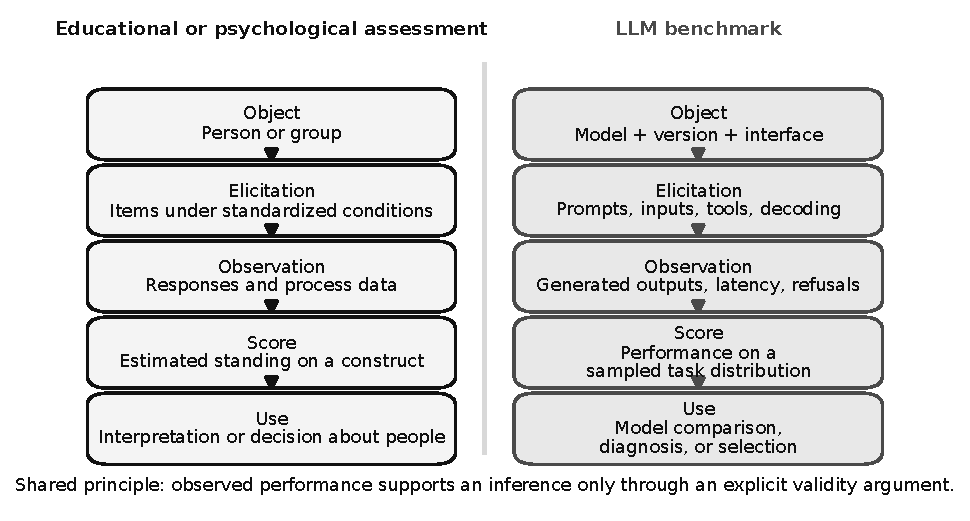
\includegraphics[width=\linewidth]{assessment_vs_benchmark.pdf}
\caption{Parallel anatomy of human assessment and LLM benchmarking. The figure is not claiming that the two enterprises are equivalent. It identifies their shared inferential structure while foregrounding the distinct object and conditions of an LLM benchmark.}
\label{fig:two-traditions}
\end{figure}

\subsection{The object is a configured system}

In most educational and psychological assessments, the object of inference is a person or group. In an LLM benchmark, ``the model'' is underspecified. Observable behavior may depend on model family, checkpoint or dated version, system message, user prompt, examples supplied in context, image resolution, enabled tools, retrieval corpus, temperature, maximum output length, and provider-side changes. The object is therefore better represented as a configured system comprising a model, version, interface, and adaptation condition. A result without this provenance may not be reproducible even when the benchmark items are public. HELM made standardization and release of raw prompts and completions central to transparent model comparison \citep{liang2022helm}; model cards and datasheets likewise emphasize documentation of intended use, provenance, and performance conditions \citep{mitchell2019modelcards,gebru2021datasheets}.

\subsection{The response process is programmable and potentially stochastic}

Human response processes vary, but a model adds distinctive sources of variability. A generative model can produce different outputs for the same input because of stochastic decoding or provider implementation. It may also return prose when a label was requested, refuse an item, call a tool, or generate malformed structured data. Prompt wording is part of the administration condition, not a neutral wrapper. Even answer-option order can change accuracy on a familiar multiple-choice benchmark \citep{gupta2024answerorder}. Consequently, a benchmark should preserve raw outputs, define parse-failure handling before analysis, and repeat administrations when stochasticity is relevant.

\subsection{Exposure can invalidate the interpretation}

In conventional testing, advance access to secure items threatens score interpretation. Public LLM benchmarks face an analogous but harder problem because model training corpora are enormous, often undisclosed, and may contain benchmark questions, answers, code, discussions, or task instructions. Contamination can therefore make memorization look like capability \citep{sainz2023contamination}. Procedures can sometimes detect exposure in black-box models with formal error control, but the general problem cannot be assumed away \citep{oren2024contamination}. Programmatic generation, newly sampled forms, private holdouts, release dates, and contamination audits are design responses, not complete guarantees.

\subsection{Scores usually describe a task distribution, not a latent trait}

A human test score is often interpreted as an estimate of standing on a psychological or educational construct, with a measurement model linking items to persons. Many LLM benchmark scores are simpler empirical summaries, such as average exact-match accuracy, mean rubric points, pass rate, preference rate, or error. They describe performance on sampled tasks under specified conditions. They do not automatically constitute a latent-variable scale, remain invariant across prompt changes, or support claims about general intelligence. The same benchmark name can also conceal a mixture of qualitatively different tasks. Data composition can affect absolute scores and model rankings, sometimes more than the choice of metric \citep{kovatchev2024transparency}. Scores from benchmarks aimed at similar capabilities may fail to concur \citep{sun2023validity}.

\subsection{The scorer may itself be a model}

Closed-form answers can often be scored deterministically. Open-ended generations require exact matching, structured rubrics, expert judgment, crowd judgment, learned metrics, or an LLM-as-a-judge. Model judges can scale evaluation, but they are measurement instruments and require validation. Agreement with human annotation varies markedly across tasks, properties, and judge models \citep{bavaresco2025judges}. A benchmark should therefore distinguish target model from judge model, preserve judge prompts and versions, and report human agreement or adjudication for a defensible sample.

The online supplement provides a detailed comparison of the two design traditions. The implication is neither that AI benchmarks are invalid nor that they must copy human testing. Rather, familiar validity principles need to be translated to a different object. Figure~\ref{fig:claim-chain} summarizes that translation. Design moves forward from an intended use to capability claims, observable evidence, tasks, and scores. Validation works backward and across the chain, asking whether each link is supported.

\begin{figure}[!htbp]
\centering
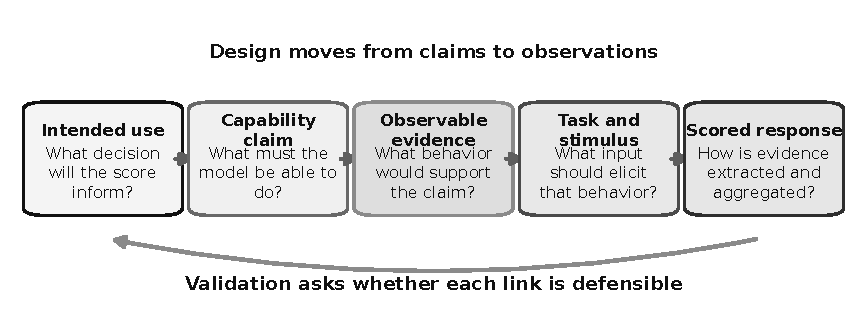
\includegraphics[width=\linewidth]{claim_evidence_chain.pdf}
\caption{The claim-to-evidence chain. A benchmark item is useful only when its response provides evidence relevant to a stated capability, and that capability is relevant to an intended use. Validation examines every link rather than treating the final score as self-interpreting.}
\label{fig:claim-chain}
\end{figure}

\section{How an LLM Benchmark Is Built}

Figure~\ref{fig:pipeline} presents an eight-stage construction process. It combines the evidentiary logic of ECBD \citep{liu2024ecbd}, the lifecycle perspective of BetterBench \citep{reuel2024betterbench}, and practices from behavioral testing, transparent evaluation, and dataset documentation. The stages are presented sequentially for teaching, although real development is iterative. The sequence is deliberately recognizable to assessment readers because benchmark construction also requires an explicit content specification, item or task review, pilot administration, scoring decisions, and revision. The analogy stops there. The benchmark object is a configured AI system, and its score usually summarizes performance over a task distribution rather than estimating a person parameter.

\begin{figure}[!htbp]
\centering
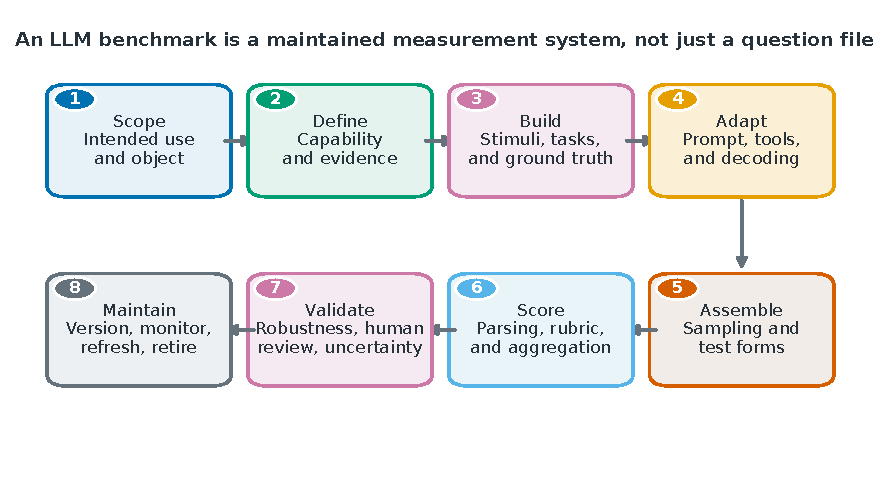
\includegraphics[width=\linewidth]{benchmark_pipeline.pdf}
\caption{An eight-stage benchmark workflow. Scope and construct decisions precede data generation; scoring is designed before claims are made; validation and maintenance are part of the benchmark rather than optional activities after publication.}
\label{fig:pipeline}
\end{figure}

\subsection{Stage 1: Specify intended use and object of evaluation}

Begin with the decision the benchmark is expected to inform. Candidate uses include scientific diagnosis of model behavior, comparison of models under a controlled research protocol, selection for a specific workflow, monitoring after deployment, or testing a hypothesized failure mode. ``Measure AI ability'' is too broad. A useful statement names users, systems, conditions, and boundaries. For example, ``IRT-Viz-Eval supports researchers and psychometric teams comparing vision-capable models for low-stakes assistance in interpreting clean, static IRT plots. It does not certify unsupervised operational decisions.''

The object of evaluation must be equally explicit. Is it a base model, chat-tuned model, hosted product, retrieval-augmented application, or agent with tools? Can it access the internet? Is the image passed at native resolution? Are prompts zero-shot, few-shot, or optimized separately for each model? A benchmark result applies to this configuration.

\subsection{Stage 2: Define capabilities and observable evidence}

Capability labels should be narrow enough to operationalize. ``Reasoning'' is not an item specification. ``Identify the lower asymptote of a dichotomous item characteristic curve'' or ``estimate response probability at a marked trait value'' is more useful. For each capability, designers should state what a successful output would look like and what competing process could produce the same answer. This is the benchmark equivalent of distinguishing construct-relevant variance from construct-irrelevant variance.

In IRT-Viz-Eval, visual psychometric interpretation is decomposed into model identification, parameter estimation, probability reading, information-peak localization, category-curve reasoning, test-level interpretation, and non-monotonic peak detection. The evidence is not merely a correct label. Numeric estimates and a brief rationale indicate which visible features the model used. The rationale is supportive process evidence, not privileged access to the model's internal computation.

\subsection{Stage 3: Construct stimuli, tasks, and ground truth}

There are three common content sources. First, experts can author and annotate items. This supports ecological relevance but is expensive and can introduce disagreement. Second, existing datasets can be repurposed. This is efficient but may import poorly documented assumptions and high contamination risk. Third, items can be generated programmatically or by models. This can produce scale, controlled variation, and exact answers, but synthetic regularities may allow shortcuts.

The content specification should cross task types with capabilities, domains, difficulty conditions, and relevant populations or contexts. Scale-development guidance likewise recommends beginning with a clear construct definition and an intentionally broad item pool before reducing it through evidence, rather than allowing available items to define the construct after the fact \citep{clarkwatson2019,hinkin1998,haynes1995,sireci1998}. Behavioral testing is useful here. CheckList distinguishes minimum functionality tests, invariance tests, and directional expectation tests rather than relying only on aggregate held-out accuracy \citep{ribeiro2020checklist}. IRT-Viz-Eval includes minimum functionality tests such as reading a probability, and invariance tests in which the same curve is rendered under different styles. Figure~\ref{fig:matrix} shows the current content matrix. Empty cells are informative because they reveal where the benchmark does not provide evidence.

\begin{figure}[!htbp]
\centering
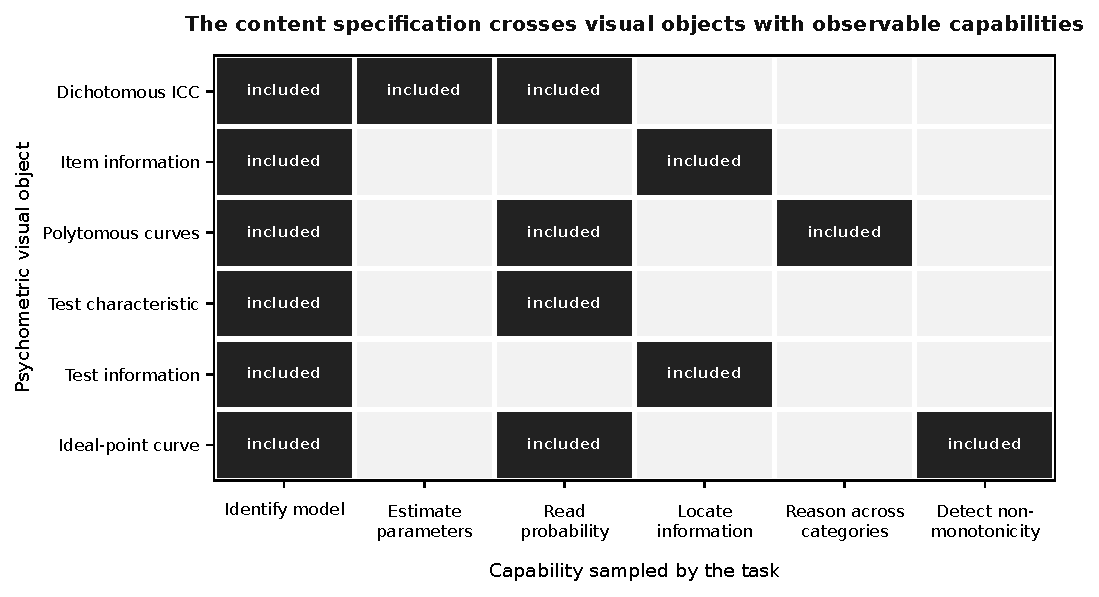
\includegraphics[width=\linewidth]{design_matrix.pdf}
\caption{IRT-Viz-Eval content specification. Rows define psychometric visual objects; columns define observable capabilities. Filled cells identify included task combinations. The matrix makes both coverage and omissions visible before a total score is calculated.}
\label{fig:matrix}
\end{figure}

Ground truth should be generated or annotated independently of the target model whenever possible. Executable tasks can be checked by running code or tests, as in SWE-bench \citep{jimenez2024swebench}. Quantitative figures can be linked to their underlying data table; ChartQA, for example, explicitly studies visual and logical reasoning over chart images and data \citep{masry2022chartqa}. IRT-Viz-Eval stores generating parameters and coordinates alongside each image, allowing exact answers to be derived rather than judged impressionistically.

\subsection{Stage 4: Standardize adaptation and elicitation}

An LLM rarely consumes a task without adaptation. The benchmark must specify the system prompt, user prompt, examples, output schema, media transformations, tool access, and decoding parameters. Adaptation can be standardized across models for comparability or tailored to each model for best-achievable performance; these answer different questions. A fair study may report both.

Prompts should be piloted for comprehension and unintended cues. In human assessment, response-process evidence asks whether respondents engage the task in the way the interpretation assumes \citep{padilla2014response}. For an LLM, the analogous evidence concerns prompt interpretation, visual access, output-schema compliance, and the distinction between a capability failure and a formatting failure. Structured output simplifies scoring but creates format-following demands. If JSON is required, researchers should report malformed-output rates rather than silently discarding them. When prompts are varied, results should be treated as a distribution over plausible administrations. Changes to answer order, formatting, or labels can function as invariance checks rather than nuisances \citep{gupta2024answerorder}.

\subsection{Stage 5: Assemble forms and choose a sampling distribution}

Benchmarks often conflate the item pool with the evaluated form. The assembly step determines which items a model actually receives and therefore what the score weights. Sampling should reflect the intended claim. Equal numbers per category estimate a balanced construct profile; prevalence-weighted sampling estimates performance under a target use distribution. Both are legitimate, but they are not interchangeable.

Designers should specify exclusions, duplicate handling, train-development-test separation, random seeds, and whether all models receive identical forms. A benchmark should be large enough to make relevant comparisons stable, but item count alone does not guarantee coverage. BetterBench found that uncertainty reporting and easy replication were uncommon even among established benchmarks \citep{reuel2024betterbench}. Bootstrap intervals over items, repeated runs, and hierarchical models can separate item, model, and administration variation.

\subsection{Stage 6: Score, aggregate, and preserve provenance}

Scoring begins with the response representation. Exact matching is transparent but brittle. Numeric tolerance bands recognize approximate visual reading. Executable validation is strong when a task has a deterministic success condition. Human rubrics support nuanced outputs but require rater training and agreement analysis. LLM judges reduce cost but need task-specific human validation \citep{bavaresco2025judges}.

Aggregation requires substantive justification. A mean can allow strength in one domain to compensate for failure in another. A worst-group or minimum-capability score encodes a different use. Accuracy and efficiency may conflict. HELM's multi-metric design illustrates why performance, robustness, fairness, calibration, toxicity, and efficiency should not automatically collapse into one rank \citep{liang2022helm}. At minimum, report total and disaggregated results, denominators, uncertainty, parse failures, refusals, and cost or latency where relevant.

\subsection{Stage 7: Validate the benchmark and its interpretation}

Validation is an accumulating argument, not a one-time coefficient. Useful evidence includes expert content review, item-level error analysis, comparison with human judgments, expected ordering of diagnostic baselines, robustness to nuisance transformations, convergence or divergence with related benchmarks, and prediction of performance in the intended workflow. Educational measurement reviews show that validity evidence is often incompletely reported across tests, especially evidence concerning consequences \citep{cizek2008,downing2003,cook2006,lane2014consequences}. Applied scale research similarly demonstrates why a single internal-consistency coefficient is not a sufficient account of structural validity and why questionable measurement practices should be made visible \citep{flake2017,flakefried2020,hussey2020}. If a future project makes trait-like claims, factor-analytic structure and invariance would require their own design and evidence rather than being assumed from a benchmark total \citep{fabrigar1999,reiser2000scale,putnick2016}. Disagreement with another benchmark is not automatically a flaw, but it requires an account of why the constructs or task distributions differ \citep{sun2023validity}.

Benchmark quality should itself be tested. Does an oracle obtain the ceiling? Does a deliberately corrupted response receive partial credit? Does a blind response perform near a meaningful floor? Do small visual changes that preserve the answer leave scores stable? Do changes intended to increase difficulty reduce performance? These checks resemble unit tests, simulation studies, and known-groups validity evidence.

\subsection{Stage 8: Maintain, refresh, and retire}

A public benchmark changes after release even if its files do not. Items can enter model training corpora, developers can optimize against the leaderboard, tasks can saturate, provider versions can drift, and intended uses can change. Dynabench treats data collection and evaluation as a dynamic human-and-model-in-the-loop process \citep{kiela2021dynabench}. A less resource-intensive project can still version releases, retain private or newly generated forms, publish change logs, monitor ceiling effects, and state retirement criteria.

Figure~\ref{fig:maintenance} makes this lifecycle explicit. A benchmark has a validity window. During this period, its evidence supports stated comparisons under documented conditions. Release is therefore the start of monitoring, not the endpoint of design.

\begin{figure}[!htbp]
\centering
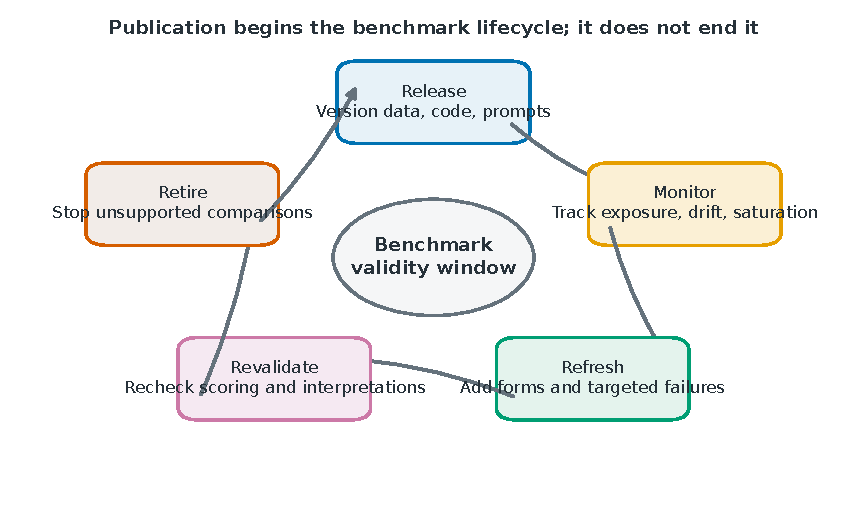
\includegraphics[width=0.92\linewidth]{maintenance_cycle.pdf}
\caption{Benchmark maintenance cycle. Monitoring addresses exposure, model drift, and saturation; refreshes require renewed validation; retirement prevents unsupported historical comparisons from being treated as current evidence.}
\label{fig:maintenance}
\end{figure}

\section{Worked Example: Constructing IRT-Viz-Eval}

\subsection{Intended use and capability model}

IRT-Viz-Eval is intended to support research on whether vision-capable language models can interpret visual artifacts used in educational measurement. It is not a certification exam for psychometricians and does not support autonomous high-stakes use. Its present domain is clean, static plots with known generating parameters. The capability claim is correspondingly bounded. Under a documented prompt and image input condition, a model can recover psychometrically relevant properties from an IRT figure and explain the visible evidence for its answer.

The substantive domain includes dichotomous 1PL, 2PL, 3PL, and 4PL item characteristic curves (ICCs); item information functions (IIFs); partial credit, generalized partial credit, and graded response category curves; test characteristic curves (TCCs); test information functions (TIFs); and a transparent non-monotonic ideal-point family. These objects have visible signatures connected to established IRT parameters \citep{rasch1960probabilistic,birnbaum1968latent,lord1980applications,samejima1969graded,andrich1978rating,muraki1992gpcm,roberts2000ggum}.

\subsection{Programmatic content and factorial rendering}

All stimuli are generated on a shared ability grid from $\theta=-4$ to $4$. Dichotomous response probabilities use

\begin{equation}
P_i(\theta)=c_i+\frac{d_i-c_i}{1+\exp[-1.7a_i(\theta-b_i)]},
\end{equation}

where $a_i$ is discrimination, $b_i$ is difficulty, $c_i$ is the lower asymptote, and $d_i$ is the upper asymptote. Item information is

\begin{equation}
I_i(\theta)=\frac{[P_i'(\theta)]^2}{P_i(\theta)[1-P_i(\theta)]}.
\end{equation}

TCCs and TIFs sum item response and information functions. Polytomous curves are produced from PCM, GPCM, and GRM probability functions. The non-monotonic stress test uses

\begin{equation}
P_i(\theta)=l_i+(u_i-l_i)\exp\left[-\frac{1}{2}\left(\frac{\theta-\delta_i}{\sigma_i}\right)^2\right].
\end{equation}

This final family is an interpretable ideal-point curve rather than a full GGUM implementation; its purpose is to test detection and localization of non-monotonicity.

Programmatic generation separates mathematical content from presentation. As Figure~\ref{fig:expansion} shows, the local validation contained 14 base mathematical stimuli. Each was rendered under six style profiles, creating 84 images and 198 linked tasks. This factorial structure makes it possible to compare responses to the same mathematical object under changed visual conditions.

\begin{figure}[!htbp]
\centering
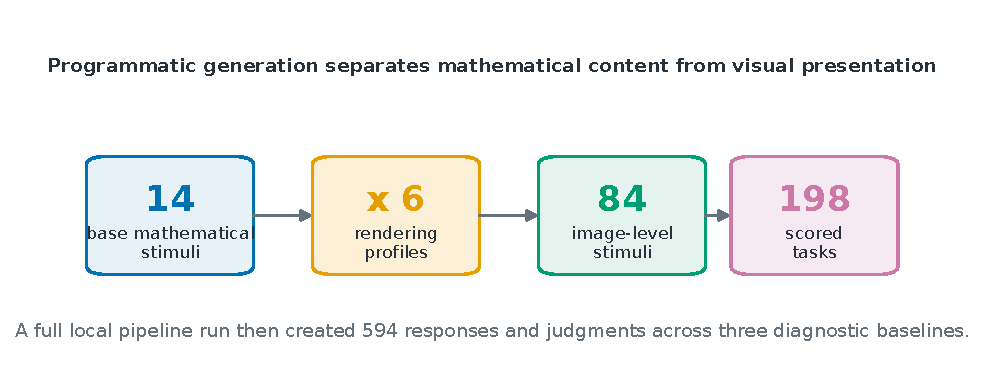
\includegraphics[width=\linewidth]{factorial_expansion.pdf}
\caption{Expansion of the local IRT-Viz-Eval validation set. The multiplication by rendering profile changes visual presentation while preserving the underlying parameters and expected answers. Different images generate different numbers of tasks, producing 198 total task records.}
\label{fig:expansion}
\end{figure}

\subsection{Invariance as a designed source of evidence}

Six profiles vary background, palette, gridline strength, tick density, legend placement, and line width. They are Matplotlib light, Seaborn white-grid, ggplot-like gray, grayscale without a grid, dark high-contrast, and lattice-like. Figure~\ref{fig:styles} displays the same 2PL ICC in all six conditions. Because the mathematical curve is held fixed, a drop associated with style is interpretable as a visual robustness failure rather than a harder IRT item. This is a benchmark analogue of an invariance test \citep{ribeiro2020checklist}.

\begin{figure}[!htbp]
\centering
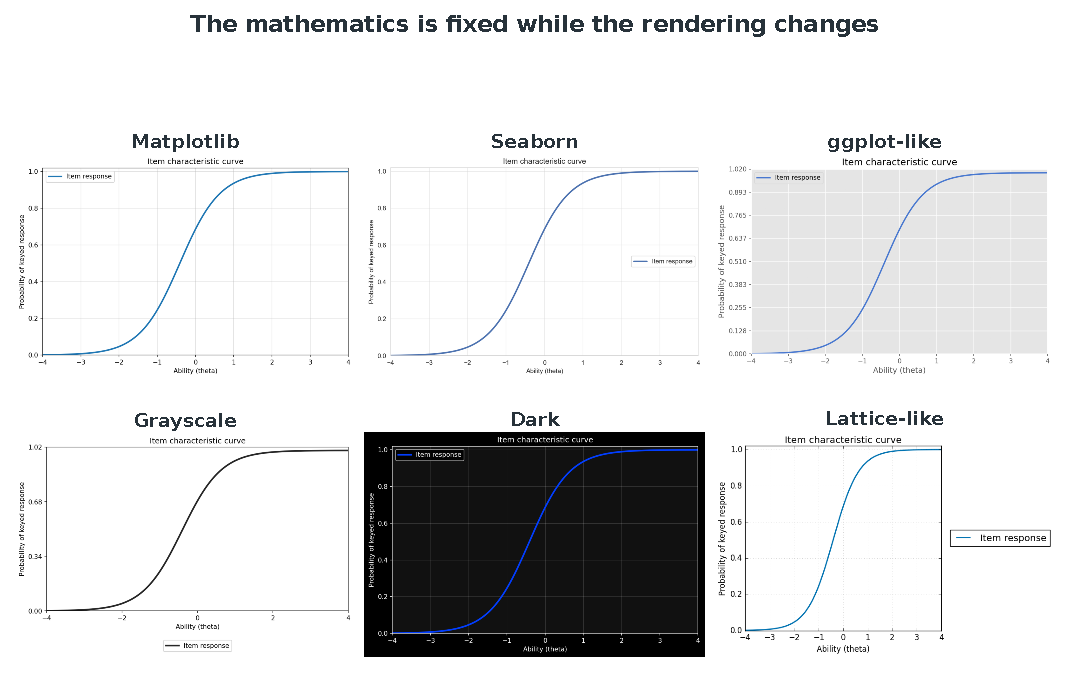
\includegraphics[width=\linewidth]{style_invariance.pdf}
\caption{Six renderings of one underlying 2PL item characteristic curve. The curve coordinates and ground truth are identical. Variation in model performance across panels therefore diagnoses sensitivity to presentation rather than psychometric content.}
\label{fig:styles}
\end{figure}

The current styles are controlled perturbations, not a representative sample of all real psychometric software. Future forms should add confidence bands, empirical noise, dense multi-item overlays, mislabeled or truncated axes, grayscale printing artifacts, and plots exported from operational systems. These additions would extend the claim from clean synthetic figures toward the figures encountered in practice.

\subsection{One benchmark instance as an evidence record}

Figure~\ref{fig:instance} shows why an item image alone is not the benchmark. A complete instance links the image to a standardized prompt, requested response schema, expected fields, field-specific thresholds, provenance, and raw output. The example asks for four dichotomous item parameters. The target output is compact JSON plus a rationale. The benchmark stores both parsed values and the original output so scoring decisions can be audited.

\begin{figure}[!htbp]
\centering
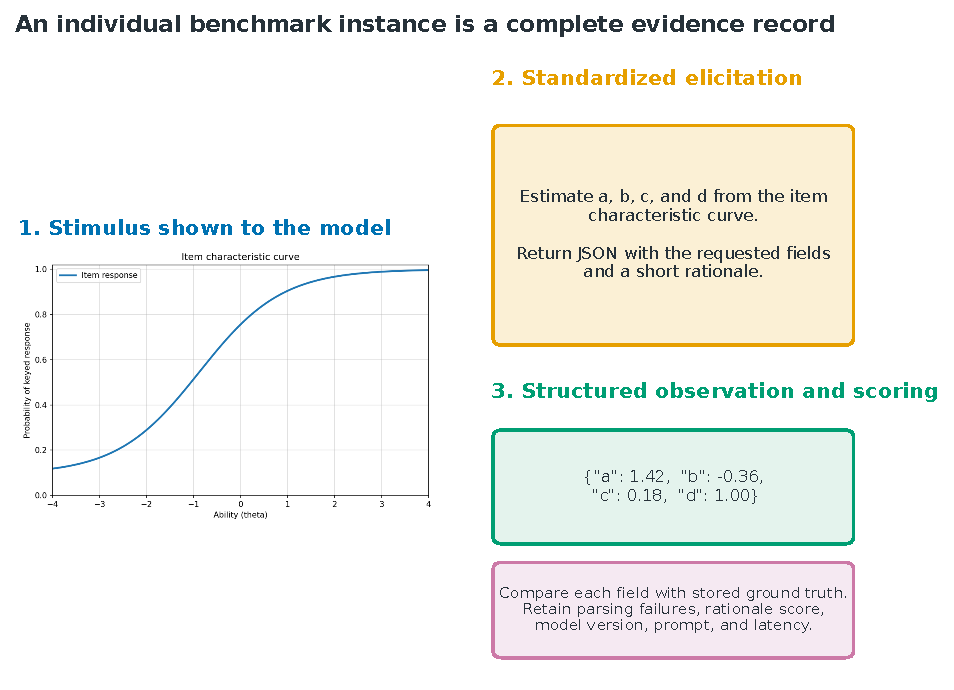
\includegraphics[width=\linewidth]{instance_anatomy.pdf}
\caption{Anatomy of an IRT-Viz-Eval instance. The stimulus, elicitation, structured observation, ground truth, and provenance together form the unit of evidence. Keeping these links prevents an image file or a score from becoming detached from its administration conditions.}
\label{fig:instance}
\end{figure}

The repository writes four linked JSONL files. A stimulus record contains the base stimulus identifier, curve family, IRT model, parameters, coordinate path, image path, and visual metadata. A task record contains the prompt, expected fields, and thresholds. A response record contains model identity, decoding settings, latency, raw output, and parsed output. A judgment record contains field-level scores, rationale score, total, normalized score, and judge provenance. JSON schemas permit automated validation and make missing provenance visible.

\subsection{Scoring design}

Categorical and integer fields receive exact-match credit after conservative normalization. Numeric fields use task-specific absolute-error bands. In the common parameter example, errors within 0.15, 0.30, and 0.50 receive 3, 2, and 1 points; larger errors receive 0. Probability-reading tasks use tighter bands of 0.05, 0.10, and 0.20. A deterministic rationale rule adds zero to two points based on the presence of prespecified psychometric terms and minimum explanatory content. This component is a reproducible proxy for visible rationale evidence, not a semantic judgment of whether every explanation is correct. Scores are normalized by the maximum available points for that task because task families request different numbers of fields.

\begin{figure}[!htbp]
\centering
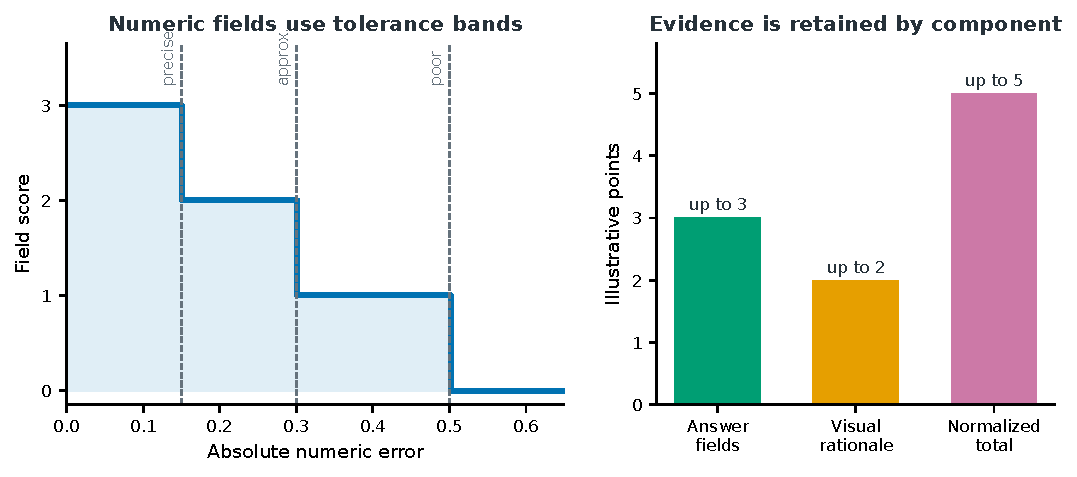
\includegraphics[width=0.94\linewidth]{scoring_logic.pdf}
\caption{Illustration of IRT-Viz-Eval scoring. The left panel shows tolerance-band scoring for a numeric field. The right panel shows why component scores are retained before normalization. Answer accuracy and rationale evidence can be inspected separately. Point totals are illustrative because the number of answer fields differs by task.}
\label{fig:scoring}
\end{figure}

Figure~\ref{fig:scoring} emphasizes two choices. First, visual reading is approximate, so a graded numeric rubric is more informative than exact string equality. Second, the normalized total is not the only result. Field errors, rationale indicators, format compliance, and task type remain available for diagnosis. A future validation study should ask experts to score a stratified response sample and estimate agreement with the deterministic rubric before replacing or supplementing it with human or LLM judgment.

\section{From Benchmark Prototype to Actual Model Administration}

\subsection{What the local baselines establish}

The local validation used seed 20260711 and one sampled base instance per model family. It produced 84 rendered stimuli and 198 tasks. Three deterministic baselines generated 594 responses. An oracle copied expected answers, a noisy baseline perturbed correct answers, and a blind baseline returned generic guesses. These are software diagnostics, not language models and not estimates of real-world performance.

The expected ordering appeared overall and within every task family. The oracle mean normalized score was 1.00, the noisy baseline was 0.73, and the blind baseline was 0.35. The complete diagnostic profile is provided in the online supplement. The result establishes that generation, parsing, field scoring, normalization, and aggregation distinguish exact, approximate, and weak responses. It does not establish content validity, human-model correspondence, or deployed-model competence.

\subsection{Choosing an API route}

Real-model responses are necessary when a claim concerns an actual system rather than benchmark mechanics. The route used to obtain those responses is part of the administration condition. Direct vendor APIs provide model-native controls; routing services expose models from several developers through one interface; dedicated endpoints provide a controlled hosted deployment; and local inference offers the greatest implementation control when hardware and open weights are available. These routes also differ in transparency, security, cost, and researcher control, concerns documented for generative-model scoring applications in educational measurement \citep{ormerod2024gpu}. OpenAI's Responses API and Google's Gemini API both accept image inputs, while Hugging Face Inference Providers routes requests to supported third-party models and compute providers through a common client \citep{openai2026vision,google2026vision,huggingface2026providers}. The online supplement compares these options and their measurement implications in detail.

Figure~\ref{fig:real-model} shows the common administration path. Each task record supplies an image, prompt, task identifier, output expectation, and scoring rule. A provider adapter sends the same model-visible content to each target system. The resulting evidence record stores the requested and returned model identifiers, access time, output limit, repetition number, latency, token usage, raw output, and any API or parsing error. The scorer operates on these stored records rather than on a live chat transcript.

\begin{figure}[!htbp]
\centering
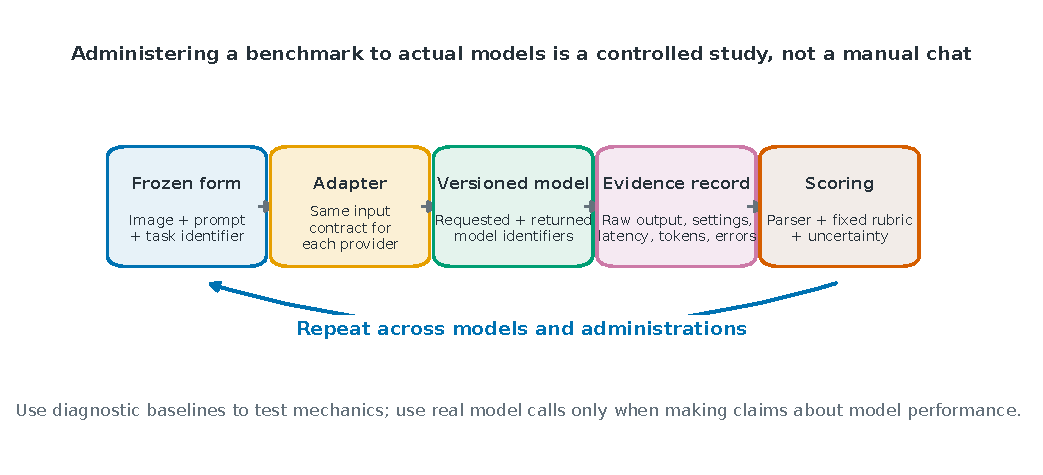
\includegraphics[width=\linewidth]{real_model_administration.pdf}
\caption{Reproducible administration of IRT-Viz-Eval to actual models. Consumer product labels such as ``ChatGPT'' are insufficient provenance; a study should record the API model identifier and returned version whenever available. Diagnostic baselines and real model calls answer different questions and should remain separate.}
\label{fig:real-model}
\end{figure}

The repository implements both an OpenAI multimodal Responses API adapter and the Hugging Face adapter used in this study. The latter used Hugging Face authentication and routing but explicitly selected the underlying inference provider in each model identifier. This distinction is important. Hugging Face supplied the common interface, model discovery, authentication, and request routing. Novita served GLM-4.5V and Qwen3-VL 30B, DeepInfra served Gemma 3 4B and Gemma 3 12B, and OVHcloud served Qwen2.5-VL 72B. A consumer subscription to ChatGPT or Gemini is not an API administration record and does not by itself supply API credits. Manual consumer-chat administration was avoided because routing, hidden instructions, media preprocessing, and versioning are difficult to audit.

\subsection{Empirical administration protocol}

The benchmark was administered on July 11--12, 2026. Five target systems were requested through Hugging Face Inference Providers. Each system received all 198 zero-shot tasks, the same PNG images and prompts, no tools, and a maximum of 1,200 completion tokens. Each prompt requested task-specific JSON plus a brief visual rationale. Unspecified decoding parameters used provider defaults. The runner used resumable JSONL output, bounded request timeouts, transient retries, and one administration per task. Exact requested and returned identifiers, compute providers, commands, and per-run logs are supplied in the online supplement.

No LLM was used as a judge. Categorical fields were scored by normalized exact match, numeric fields by prespecified tolerance bands, and rationale evidence by the fixed rule described earlier. The primary model score was the unweighted mean of the 198 task-normalized scores. To represent uncertainty over sampled mathematical content, 95\% intervals were calculated from 10,000 cluster-bootstrap draws over the 14 base stimuli. The paired interval for the model difference resampled the same base-stimulus clusters. These intervals do not represent within-model sampling variability because only one response per task was collected.

\subsection{Five-model results}

All five systems completed 198 unique tasks without a recorded API error after deduplication. Qwen2.5-VL 72B had the highest mean task-normalized score (.719, 95\% cluster-bootstrap CI [.656, .788]), followed by Qwen3-VL 30B (.704, [.643, .774]). GLM-4.5V (.628, [.536, .727]) and Gemma 3 4B (.629, [.587, .673]) were nearly tied, while Gemma 3 12B scored .600 ([.549, .653]). The paired intervals indicate that the two Qwen systems were not clearly separated, whereas both were above the Gemma and GLM systems in several pairwise comparisons under this task distribution. These are descriptive comparisons from one administration, not stable model traits. Table~\ref{tab:overall-results} also shows a consequential aggregation choice. Raw rubric points give more weight to tasks with more requested fields, whereas task normalization gives every task equal weight.

\begin{table}[!htbp]
\centering
\small
\caption{Overall scores and administration diagnostics for the complete 198-task runs.}
\label{tab:overall-results}
\begin{tabular}{@{}lccccc@{}}
\toprule
Model & Mean score & 95\% CI & Points & Empty output & Median latency \\
\midrule
Qwen2.5-VL 72B & .719 & [.656, .788] & 905/1,236 & 0.0\% & 3.48 s \\
Qwen3-VL 30B & .704 & [.643, .774] & 873/1,236 & 0.0\% & 2.25 s \\
Gemma 3 4B & .629 & [.587, .673] & 742/1,236 & 0.0\% & 2.14 s \\
GLM-4.5V & .628 & [.536, .727] & 668/1,236 & 16.7\% & 13.79 s \\
Gemma 3 12B & .600 & [.549, .653] & 782/1,236 & 0.0\% & 3.04 s \\
\bottomrule
\end{tabular}
\end{table}

Operationally, the routed systems were not equivalent. GLM produced visible text for 165 tasks and parseable JSON for 152; Gemma 3 4B, Gemma 3 12B, and Qwen2.5-VL 72B produced nonempty, parseable JSON for all 198, while Qwen3-VL 30B produced parseable JSON for 194. Median latency ranged from 2.14 seconds for Gemma 3 4B to 13.79 seconds for GLM-4.5V. Provider-reported total token counts ranged from 84,523 for Gemma 3 12B to 342,107 for GLM-4.5V. These values describe the routed systems under this protocol, not immutable properties of the model weights, because providers can differ in image tokenization, reasoning-token accounting, serving hardware, and defaults.

\begin{figure}[!htbp]
\centering
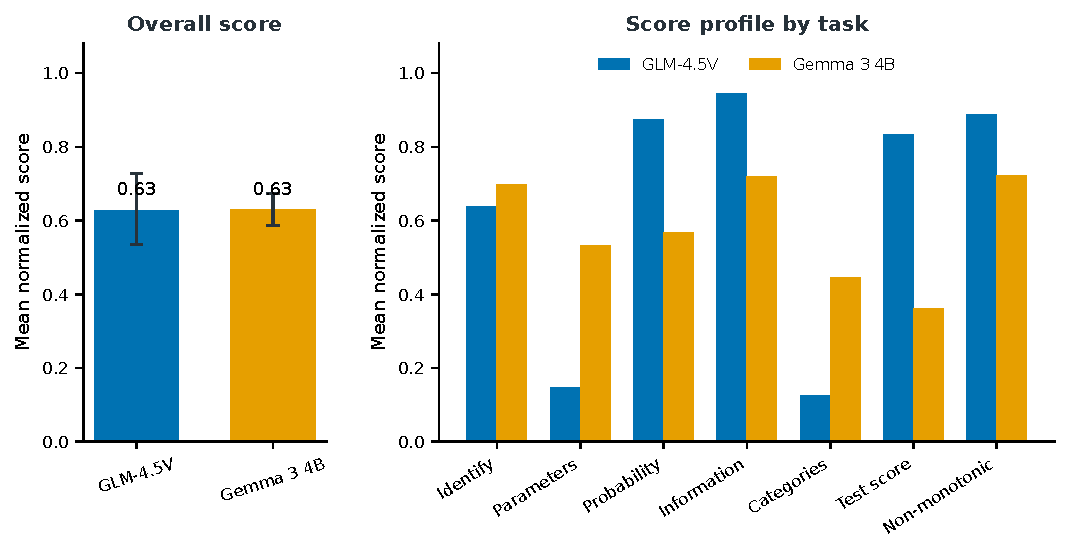
\includegraphics[width=\linewidth]{empirical_model_results.pdf}
\caption{Complete five-model results. Overall bars show mean task-normalized scores with 95\% cluster-bootstrap intervals over base mathematical stimuli. Task-level profiles reveal that overall ordering is only one part of the benchmark evidence.}
\label{fig:empirical-results}
\end{figure}

The overall scores concealed substantial profile differences (Figure~\ref{fig:empirical-results}). Qwen2.5-VL 72B was strongest on information peaks (.979), test expected scores (1.000), and non-monotonic peaks (.963); Qwen3-VL 30B was strongest on model identification (.730) and was close to Qwen2.5-VL 72B on information peaks (.950). GLM-4.5V remained strongest among the smaller systems on probability reading (.873) and information peaks (.946), while Gemma 3 12B led parameter estimation (.675). Gemma 3 4B led category-curve reasoning among the Gemma systems (.444), but the Qwen systems were higher (.597 and .646). The task profile therefore supplies information that a single total suppresses. Exact task-type values are provided in the online supplement. These are descriptive comparisons from one administration; they identify hypotheses for repeated evaluation rather than stable model traits.

Style scores varied within a narrower range than substantive task profiles for all five systems. The ranges were .599--.663 for GLM, .608--.666 for Gemma 4B, .555--.644 for Gemma 12B, .683--.729 for Qwen3-VL 30B, and .687--.746 for Qwen2.5-VL 72B. This descriptive consistency is encouraging evidence that no single plotting theme determined the overall result, but six synthetic styles are not a sample of all operational graphics. Curve-family profiles differed more sharply, especially for test-characteristic and unfolding tasks. The online supplement provides the complete rendering-profile and curve-family figure. This is why style robustness should be reported alongside, rather than substituted for, content coverage.

\section{Validity Threats in LLM Benchmarking}

Figure~\ref{fig:threats} locates five threats along the path from stimulus to claim. The diagram is deliberately causal in spirit. An observed score can be altered by factors introduced before, during, or after model generation.

\begin{figure}[!htbp]
\centering
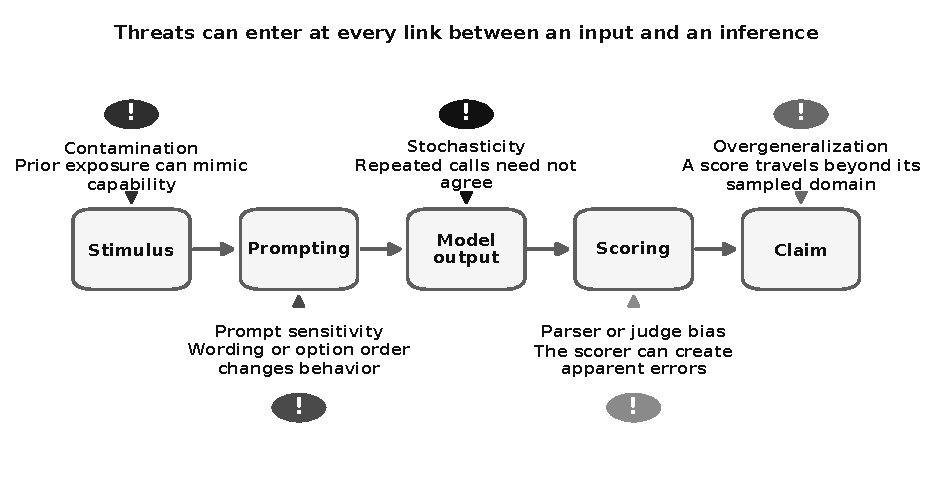
\includegraphics[width=\linewidth]{threats_to_inference.pdf}
\caption{Threats to benchmark inference. Contamination affects the relation between stimulus and capability; prompt sensitivity affects elicitation; stochasticity affects observed output; parser or judge bias affects scoring; overgeneralization affects the interpretation attached to the score.}
\label{fig:threats}
\end{figure}

\subsection{Contamination and shortcut learning}

Prior exposure can occur at the level of task instructions, raw text or images, labels, code, or public discussions \citep{sainz2023contamination}. Programmatic generation reduces exact-item exposure but does not prevent a model from learning the generating template. Designers should therefore vary parameters and rendering conditions, keep some generators or forms private where appropriate, record release dates, and avoid claims that require proving complete non-exposure.

Shortcuts can arise even without contamination. A model may infer the answer from filenames, alt text, legend labels, repeated color mappings, or template regularities. Benchmark packaging should remove answer-bearing metadata from the model-visible input. Counterbalanced and adversarial variants can test whether a purported capability survives removal of the cue.

\subsection{Prompt and interface sensitivity}

The prompt determines what behavior is elicited. A model can fail because it lacks the target capability, misunderstands an instruction, cannot emit the requested format, or follows a conflicting system policy. These are different findings. Reporting multiple plausible prompts and invalid-output rates helps distinguish them. A benchmark intended to compare model products should also treat provider preprocessing and tool access as part of the product, while a benchmark intended to compare base capabilities may disable them.

\subsection{Stochasticity and version drift}

A single API response is one draw from a configured system. Repeated runs reveal whether model rankings are stable or depend on sampling. Hosted systems may change without a new public name. Access dates, model identifiers, raw outputs, and periodic anchor-item reruns are therefore essential. Historical scores should not be pooled across silent model versions as if they were measurements of one fixed object.

\subsection{Scoring and judge error}

Parsers can mark semantically correct outputs wrong, while permissive extraction can reward extraneous or contradictory text. LLM judges may exhibit task-specific disagreement with people and each other \citep{bavaresco2025judges}. Deterministic scoring should be preferred when ground truth is structured. When judgment is necessary, designers should publish the rubric, blind or randomize comparison order, estimate agreement with relevant human experts, retain individual judgments, and specify adjudication.

\subsection{Overgeneralization and consequential validity}

Benchmark results often travel farther than their design. A score on synthetic IRT plots does not establish competence with empirical calibration reports, psychometric decision making, or the consequences of wrong advice. Raji and colleagues' critique of ``general'' benchmarks is a reminder that dataset breadth is not a license for unbounded claims \citep{raji2021everything}; consequences evidence similarly asks what follows when scores are used for decisions \citep{lane2014consequences}. The defensible interpretation should name the sampled content, model configuration, score rule, date, and intended use. Any model-selection decision should add use-specific validation rather than rely on a broad leaderboard alone.

\section{A Reusable Recipe for Social Science Benchmark Projects}

For a social science team beginning an LLM evaluation, the following sequence is a practical minimum.

\begin{enumerate}
\item Write one paragraph naming the decision, users, model system, context, and claims that are out of scope.
\item Create a construct map with narrow capabilities and observable behaviors; have subject-matter experts review it.
\item Build a content matrix crossing capabilities with domains, task types, difficulty, and nuisance transformations.
\item Choose an item source and ground-truth process; retain provenance and separate target-model generation from answer creation.
\item Pilot prompts and response schemas on several model families; freeze administration rules before comparison.
\item Define form assembly and analysis denominators, including invalid outputs and refusals.
\item Implement scoring with unit tests, diagnostic baselines, and human validation for judgment-based components.
\item Report disaggregated results and uncertainty; inspect errors before ranking models.
\item Publish documentation, raw outputs where permitted, code, version identifiers, known limitations, and maintenance plans.
\item Refresh, revalidate, or retire when exposure, saturation, model drift, or new intended uses undermine the original argument.
\end{enumerate}

This recipe is intentionally closer to assessment design than to downloading a test set and calculating accuracy. It also remains different from human psychometrics. A team need not fit an IRT model to every benchmark or treat models as people. The transferable insight is evidentiary discipline. Define the claim, design observations that bear on it, standardize the elicitation, quantify uncertainty, and constrain the interpretation.

\section{Discussion}

LLM benchmarking and social science measurement have much to offer one another. Benchmark developers contribute practices for executable evaluation, large-scale automation, adversarial testing, and rapid iteration. Social scientists contribute theories of constructs, response processes, validity arguments, fairness, sampling, and consequences. Scale-development research adds a practical discipline of specifying the content domain, reviewing candidate indicators, piloting administration, examining structure, and revising before broad use \citep{boateng2018,simms2008}. ECBD demonstrates that this exchange is already possible \citep{liu2024ecbd}. BetterBench's lifecycle analysis similarly shows that benchmark quality depends on design, implementation, documentation, maintenance, and eventual retirement rather than predictive performance alone \citep{reuel2024betterbench}.

IRT-Viz-Eval illustrates the benefits of this combined perspective. Programmatic generation provides exact answers; factorial rendering supports controlled robustness evidence; structured records preserve provenance; field-level scoring supports error analysis; and diagnostic baselines test mechanics. The five real-model administrations add a second lesson. Qwen2.5-VL 72B and Qwen3-VL 30B ranked above the other systems on the aggregate task distribution, but the task profiles crossed repeatedly; the smallest Gemma system was nearly tied with GLM overall; GLM had a 16.7\% empty-output rate; median latency differed by more than sixfold; and raw-point and task-normalized aggregation answer different questions. Benchmark construction decisions were therefore not background details; they changed what a comparison would mean.

The validity argument remains bounded. The benchmark samples clean synthetic plots, five routed systems and one response per task were observed, provider defaults were not fully harmonized, the rationale rule needs expert validation, and the six style profiles do not represent the ecology of operational psychometric graphics. The cluster-bootstrap intervals reflect variation across 14 mathematical base stimuli, not model stochasticity, future provider drift, or uncertainty in scoring. The benchmark has not been developed as a validated latent-trait scale for AI systems, and these empirical results do not establish that any model is suitable for unsupervised psychometric decisions. The educational and psychological measurement literature is therefore used here to improve benchmark construction and score interpretation, not to imply that the present benchmark has completed the evidence needed for psychometric claims about model ability.

The next validation phase should repeat administrations, counterbalance plausible prompts, and obtain blinded expert scores for a stratified response sample. Content extensions should include empirical estimation noise, confidence bands, differential item functioning plots, item-fit diagnostics, score-report visualizations, and accessibility conditions. An external study could then test whether benchmark performance predicts quality on authentic psychometric review tasks.

\section{Conclusion}

An LLM benchmark is best understood as a maintained measurement system. Its data are only one component. The prompts define elicitation, the model configuration defines the object, the parser or judge defines the observation, the assembly rule defines the sampled domain, and the validity argument defines what the score can mean. These features distinguish benchmarking from conventional educational and psychological assessment while preserving a shared commitment to evidence-based interpretation.

For social scientists, the practical lesson is straightforward. Do not begin or end with a leaderboard. Begin with an intended use and a defensible capability claim. Build backward to the evidence and tasks, then move forward through standardized administration, scoring, validation, reporting, and maintenance. The empirical demonstration showed why. Five systems differed in overall score, task profile, output validity, latency, and aggregation behavior. IRT-Viz-Eval provides one complete implementation of this benchmark-development process and a bounded foundation for studying multimodal interpretation of psychometric graphics. Its purpose is to teach how such a benchmark is built and administered, not to declare that the benchmark itself is a finished psychometric scale for AI.

\ifprintappendix
\clearpage
\appendix

\section{Benchmark Construction Checklist}

\begin{longtable}{p{0.18\linewidth}p{0.76\linewidth}}
\caption{Questions to answer before releasing or using an LLM benchmark.}\label{tab:checklist}\\
\toprule
Stage & Required questions \\
\midrule
\endfirsthead
\toprule
Stage & Required questions \\
\midrule
\endhead
Intended use & Who will use the result? What decision will it inform? What interpretations and uses are explicitly unsupported? \\
Object & What exact model, version, interface, tools, retrieval sources, and provider settings are being evaluated? Can these change during the study? \\
Capability & What narrow behavior is claimed? Which alternative processes could produce the same observed answer? \\
Content & What domains, task types, difficulty levels, languages, groups, and modalities are sampled? Which cells are absent? \\
Ground truth & Who or what creates the reference answer? Is it independently checked? How are ambiguity and disagreement represented? \\
Adaptation & What system prompt, user prompt, examples, image transformations, output schema, decoding settings, and retries are used? \\
Assembly & How are tasks selected and weighted? Are forms identical across models? What seed and exclusion rules are used? \\
Scoring & How are raw outputs parsed? How are refusals, multiple answers, malformed outputs, and missing fields scored? \\
Judgment & If people or LLMs judge outputs, what rubric, training, blinding, agreement, adjudication, and judge provenance are used? \\
Uncertainty & What varies across items, repeated calls, prompts, forms, models, and judges? Which interval or model represents that variation? \\
Robustness & Which meaning-preserving changes should leave scores stable? Which difficulty manipulations should change scores predictably? \\
Contamination & Could items, answers, templates, or code have entered training data? What evidence and mitigation are available? \\
Documentation & Are data provenance, licenses, model versions, prompts, raw outputs, code, exclusions, costs, and limitations documented? \\
Maintenance & Who owns updates? How will exposure, drift, and saturation be monitored? What triggers a new version or retirement? \\
\bottomrule
\end{longtable}

\section{IRT-Viz-Eval Task Families}

\begin{table}[H]
\centering
\caption{Current task families and primary evidence fields.}
\begin{tabularx}{\linewidth}{>{\raggedright\arraybackslash}p{0.25\linewidth}Y>{\raggedright\arraybackslash}p{0.24\linewidth}}
\toprule
Task family & Observable response & Primary scoring \\
\midrule
Model identification & IRT model or curve family plus visual rationale & Exact categorical match + rationale \\
Parameter estimation & $a$, $b$, $c$, $d$ where applicable & Numeric tolerance bands \\
Probability reading & $P(\theta)$ at a specified location & Numeric tolerance bands \\
Information peak & Peak location and height & Numeric tolerance bands \\
Category reasoning & Category count, modal category, expected score & Integer, categorical, and numeric fields \\
Test characteristic & Form length and expected raw score & Integer and numeric fields \\
Non-monotonic peak & Non-monotonicity, peak location, peak probability & Categorical and numeric fields \\
\bottomrule
\end{tabularx}
\end{table}

\section{Linked Data Schema}

Each line is a JSON object with a stable identifier. The joins are as follows.

\begin{center}
\texttt{stimulus\_id} $\rightarrow$ \texttt{task\_id} $\rightarrow$ \texttt{response\_id} $\rightarrow$ \texttt{judgment\_id}.
\end{center}

\begin{table}[H]
\centering
\caption{Minimum fields retained in each benchmark artifact.}
\begin{tabularx}{\linewidth}{p{0.18\linewidth}Y}
\toprule
Artifact & Core fields \\
\midrule
Stimulus & Base and rendered identifiers; model family; mathematical parameters; ground truth; coordinate path; image path; style, axes, palette, legend, size, and render engine \\
Task & Task type; prompt; prompt-template identifier; expected answer fields; field types; numeric thresholds; rubric; image link \\
Response & Target model and version; system and user prompts; decoding settings; seed; access time; latency; raw output; parsed output; parser version \\
Judgment & Response link; field-level errors and scores; rationale score; total and maximum score; normalized score; judge type, version, prompt, and timestamp \\
\bottomrule
\end{tabularx}
\end{table}

\section{Reporting Template for an Empirical Model Study}

An empirical paper using this benchmark should report the following information.

\begin{enumerate}
\item benchmark release, generator version, date generated, item count, task count, and form seed;
\item every target model's provider, identifier, access date, modality support, context limit, and tool configuration;
\item full system and user prompts, examples, response schema, image preprocessing, decoding, retries, and repetitions;
\item primary and secondary outcomes, aggregation weights, invalid-output policy, uncertainty procedure, and multiplicity handling;
\item deterministic scorer version and, if applicable, judge model, prompt, order randomization, human validation sample, and agreement;
\item overall and disaggregated results by task, curve family, style, and base stimulus, including denominators and confidence intervals;
\item parse failures, refusals, latency, token use, cost, exclusions, and missing data;
\item contamination considerations, benchmark limitations, intended interpretation, unsupported uses, and a link to raw outputs where licensing permits.
\end{enumerate}

\section{Reproducibility Resources}

The repository includes a one-command local pipeline, source modules for psychometric generation and rendering, JSON schemas, target and judge prompts, generated stimuli and task records, diagnostic responses and judgments, analysis tables, and the script that generated every figure in this article. The local command follows.

\begin{verbatim}
bash scripts/run_local_benchmark.sh
\end{verbatim}

After installing the optional provider dependency and authenticating locally, administer a small Hugging Face pilot with the following command.

\begin{verbatim}
PYTHONPATH=src python3 -m irt_viz_eval.cli run-huggingface \
  --models MODEL_ID:PROVIDER --limit 10 \
  --request-timeout 180 --max-retries 3
\end{verbatim}

The adapter supports task limits, repeated administrations, resumable output, bounded timeouts, transient retries, and per-task progress. The repository also includes an OpenAI Responses API adapter; the shared response schema permits future Gemini or local-runtime adapters without changing the task and judgment records. Model identifiers are supplied at runtime because provider availability changes. Credentials are never stored in the repository. The empirical preparation script deduplicates response identifiers, requires complete 198-task coverage, applies the deterministic scorer, and produces the published tables and cluster-bootstrap intervals.

Regenerate the paper figures with the following command.

\begin{verbatim}
python3 paper/generate_figures.py
\end{verbatim}

Regenerate the complete empirical outputs used in this manuscript after the five raw response files are present with the following commands.

\begin{verbatim}
PYTHONPATH=src python3 paper/prepare_empirical_results.py
PYTHONPATH=src python3 paper/generate_supplement.py
\end{verbatim}

Downloaded source articles used during manuscript development are not redistributed. Persistent publisher and repository locations are supplied in the reference list where available.

\fi
\section{Declarations}

\noindent\textbf{Data and code availability.} Code and benchmark materials are available at \url{https://github.com/pbotter42/IRT-Viz-Eval}. The exact response records, judgments, analysis outputs, and figure-generation materials used for this preprint are included in the accompanying reproducibility archive.

\noindent\textbf{Ethics statement.} Ethics review was not required because the study used synthetic benchmark stimuli and model-generated responses and involved no human participants or personal data.

\noindent\textbf{Funding.} This research received no external funding.

\noindent\textbf{Competing interests.} The author declares no competing interests.

\noindent\textbf{Generative AI disclosure.} Generative AI tools assisted with editing, code development, literature discovery, and figure development. The author reviewed the underlying sources, tested the code, verified the manuscript and references, and accepts responsibility for the final work.

\bibliographystyle{apalike}
\bibliography{references}

\end{document}
